\documentclass[12pt,twoside]{article}
\usepackage[utf8]{inputenc}
\newcommand{\reporttitle}{Robotic Finger}
\newcommand{\reportauthor}{José Daniel Badilla Umaña \\Luis Alonso Barboza Artavia  \\Jason Josue Leitón Jiménez\\ Carlos Peralta Coto}
\newcommand{\reporttype}{Operatives Systems}
\newcommand{\cid}{your college-id number}

% include files that load packages and define macros
%%%%%%%%%%%%%%%%%%%%%%%%%%%%%%%%%%%%%%%%%
% University Assignment Title Page 
% LaTeX Template
% Version 1.0 (27/12/12)
%
% This template has been downloaded from:
% http://www.LaTeXTemplates.com
%
% Original author:
% WikiBooks (http://en.wikibooks.org/wiki/LaTeX/Title_Creation)
%
% License:
% CC BY-NC-SA 3.0 (http://creativecommons.org/licenses/by-nc-sa/3.0/)
% 
% Instructions for using this template:
% This title page is capable of being compiled as is. This is not useful for 
% including it in another document. To do this, you have two options: 
%
% 1) Copy/paste everything between \begin{document} and \end{document} 
% starting at \begin{titlepage} and paste this into another LaTeX file where you 
% want your title page.
% OR
% 2) Remove everything outside the \begin{titlepage} and \end{titlepage} and 
% move this file to the same directory as the LaTeX file you wish to add it to. 
% Then add \input{./title_page_1.tex} to your LaTeX file where you want your
% title page.
%
%----------------------------------------------------------------------------------------
%	PACKAGES AND OTHER DOCUMENT CONFIGURATIONS
%----------------------------------------------------------------------------------------
\usepackage{ifxetex}
\usepackage{textpos}
%\usepackage{natbib}
\usepackage{kpfonts}
\usepackage[a4paper,hmargin=2.8cm,vmargin=2.0cm,includeheadfoot]{geometry}
\usepackage{ifxetex}
\usepackage{stackengine}
\usepackage{tabularx,longtable,multirow,subfigure,caption}%hangcaption
\usepackage{fncylab} %formatting of labels
\usepackage{fancyhdr}
\usepackage{color}
\usepackage[tight,ugly]{units}
\usepackage{url}
\usepackage{float}
\usepackage[english]{babel}
\usepackage{amsmath}
\usepackage{graphicx}
\usepackage[colorinlistoftodos]{todonotes}
\usepackage{dsfont}
\usepackage{epstopdf} % automatically replace .eps with .pdf in graphics
%\usepackage{natbib}
\usepackage{backref}
\usepackage{array}
\usepackage{latexsym}
\usepackage{etoolbox}

\usepackage{enumerate} % for numbering with [a)] format 



\ifxetex
\usepackage{fontspec}
\setmainfont[Scale=.8]{OpenDyslexic-Regular}
\else
\usepackage[pdftex,pagebackref,hypertexnames=false,colorlinks]{hyperref} % provide links in pdf
\hypersetup{pdftitle={},
  pdfsubject={}, 
  pdfauthor={\reportauthor},
  pdfkeywords={}, 
  pdfstartview=FitH,
  pdfpagemode={UseOutlines},% None, FullScreen, UseOutlines
  bookmarksnumbered=true, bookmarksopen=true, colorlinks,
    citecolor=black,%
    filecolor=black,%
    linkcolor=black,%
    urlcolor=black}
\usepackage[all]{hypcap}
\fi

\usepackage{tcolorbox}

% various theorems
\usepackage{ntheorem}
\theoremstyle{break}
\newtheorem{lemma}{Lemma}
\newtheorem{theorem}{Theorem}
\newtheorem{remark}{Remark}
\newtheorem{definition}{Definition}
\newtheorem{proof}{Proof}

% example-environment
\newenvironment{example}[1][]
{ 
\vspace{4mm}
\noindent\makebox[\linewidth]{\rule{\hsize}{1.5pt}}
\textbf{Example #1}\\
}
{ 
\noindent\newline\makebox[\linewidth]{\rule{\hsize}{1.0pt}}
}



%\renewcommand{\rmdefault}{pplx} % Palatino
% \renewcommand{\rmdefault}{put} % Utopia

\ifxetex
\else
\renewcommand*{\rmdefault}{bch} % Charter
\renewcommand*{\ttdefault}{cmtt} % Computer Modern Typewriter
%\renewcommand*{\rmdefault}{phv} % Helvetica
%\renewcommand*{\rmdefault}{iwona} % Avant Garde
\fi

\setlength{\parindent}{0em}  % indentation of paragraph

\setlength{\headheight}{14.5pt}
\pagestyle{fancy}
\fancyfoot[ER,OL]{\thepage}%Page no. in the left on
                                %odd pages and on right on even pages
\fancyfoot[OC,EC]{\sffamily }
\renewcommand{\headrulewidth}{0.1pt}
\renewcommand{\footrulewidth}{0.1pt}
\captionsetup{margin=10pt,font=small,labelfont=bf}


%--- chapter heading

\def\@makechapterhead#1{%
  \vspace*{10\p@}%
  {\parindent \z@ \raggedright %\sffamily
        %{\Large \MakeUppercase{\@chapapp} \space \thechapter}
        %\\
        %\hrulefill
        %\par\nobreak
        %\vskip 10\p@
    \interlinepenalty\@M
    \Huge \bfseries 
    \thechapter \space\space #1\par\nobreak
    \vskip 30\p@
  }}

%---chapter heading for \chapter*  
\def\@makeschapterhead#1{%
  \vspace*{10\p@}%
  {\parindent \z@ \raggedright
    \sffamily
    \interlinepenalty\@M
    \Huge \bfseries  
    #1\par\nobreak
    \vskip 30\p@
  }}
  



% %%%%%%%%%%%%% boxit
\def\Beginboxit
   {\par
    \vbox\bgroup
	   \hrule
	   \hbox\bgroup
		  \vrule \kern1.2pt %
		  \vbox\bgroup\kern1.2pt
   }

\def\Endboxit{%
			      \kern1.2pt
		       \egroup
		  \kern1.2pt\vrule
		\egroup
	   \hrule
	 \egroup
   }	

\newenvironment{boxit}{\Beginboxit}{\Endboxit}
\newenvironment{boxit*}{\Beginboxit\hbox to\hsize{}}{\Endboxit}



\allowdisplaybreaks

\makeatletter
\newcounter{elimination@steps}
\newcolumntype{R}[1]{>{\raggedleft\arraybackslash$}p{#1}<{$}}
\def\elimination@num@rights{}
\def\elimination@num@variables{}
\def\elimination@col@width{}
\newenvironment{elimination}[4][0]
{
    \setcounter{elimination@steps}{0}
    \def\elimination@num@rights{#1}
    \def\elimination@num@variables{#2}
    \def\elimination@col@width{#3}
    \renewcommand{\arraystretch}{#4}
    \start@align\@ne\st@rredtrue\m@ne
}
{
    \endalign
    \ignorespacesafterend
}
\newcommand{\eliminationstep}[2]
{
    \ifnum\value{elimination@steps}>0\leadsto\quad\fi
    \left[
        \ifnum\elimination@num@rights>0
            \begin{array}
            {@{}*{\elimination@num@variables}{R{\elimination@col@width}}
            |@{}*{\elimination@num@rights}{R{\elimination@col@width}}}
        \else
            \begin{array}
            {@{}*{\elimination@num@variables}{R{\elimination@col@width}}}
        \fi
            #1
        \end{array}
    \right]
    & 
    \begin{array}{l}
        #2
    \end{array}
    &%                                    moved second & here
    \addtocounter{elimination@steps}{1}
}
\makeatother

%% Fast macro for column vectors
\makeatletter  
\def\colvec#1{\expandafter\colvec@i#1,,,,,,,,,\@nil}
\def\colvec@i#1,#2,#3,#4,#5,#6,#7,#8,#9\@nil{% 
  \ifx$#2$ \begin{bmatrix}#1\end{bmatrix} \else
    \ifx$#3$ \begin{bmatrix}#1\\#2\end{bmatrix} \else
      \ifx$#4$ \begin{bmatrix}#1\\#2\\#3\end{bmatrix}\else
        \ifx$#5$ \begin{bmatrix}#1\\#2\\#3\\#4\end{bmatrix}\else
          \ifx$#6$ \begin{bmatrix}#1\\#2\\#3\\#4\\#5\end{bmatrix}\else
            \ifx$#7$ \begin{bmatrix}#1\\#2\\#3\\#4\\#5\\#6\end{bmatrix}\else
              \ifx$#8$ \begin{bmatrix}#1\\#2\\#3\\#4\\#5\\#6\\#7\end{bmatrix}\else
                 \PackageError{Column Vector}{The vector you tried to write is too big, use bmatrix instead}{Try using the bmatrix environment}
              \fi
            \fi
          \fi
        \fi
      \fi
    \fi
  \fi 
}  
\makeatother

\robustify{\colvec}

%%% Local Variables: 
%%% mode: latex
%%% TeX-master: "notes"
%%% End: 
 % various packages needed for maths etc.
% quick way of adding a figure
\newcommand{\fig}[3]{
 \begin{center}
 \scalebox{#3}{\includegraphics[#2]{#1}}
 \end{center}
}

%\newcommand*{\point}[1]{\vec{\mkern0mu#1}}
\newcommand{\ci}[0]{\perp\!\!\!\!\!\perp} % conditional independence
\newcommand{\point}[1]{{#1}} % points 
\renewcommand{\vec}[1]{{\boldsymbol{{#1}}}} % vector
\newcommand{\mat}[1]{{\boldsymbol{{#1}}}} % matrix
\newcommand{\R}[0]{\mathds{R}} % real numbers
\newcommand{\Z}[0]{\mathds{Z}} % integers
\newcommand{\N}[0]{\mathds{N}} % natural numbers
\newcommand{\nat}[0]{\mathds{N}} % natural numbers
\newcommand{\Q}[0]{\mathds{Q}} % rational numbers
\ifxetex
\newcommand{\C}[0]{\mathds{C}} % complex numbers
\else
\newcommand{\C}[0]{\mathds{C}} % complex numbers
\fi
\newcommand{\tr}[0]{\text{tr}} % trace
\renewcommand{\d}[0]{\mathrm{d}} % total derivative
\newcommand{\inv}{^{-1}} % inverse
\newcommand{\id}{\mathrm{id}} % identity mapping
\renewcommand{\dim}{\mathrm{dim}} % dimension
\newcommand{\rank}[0]{\mathrm{rk}} % rank
\newcommand{\determ}[1]{\mathrm{det}(#1)} % determinant
\newcommand{\scp}[2]{\langle #1 , #2 \rangle}
\newcommand{\kernel}[0]{\mathrm{ker}} % kernel/nullspace
\newcommand{\img}[0]{\mathrm{Im}} % image
\newcommand{\idx}[1]{{(#1)}}
\DeclareMathOperator*{\diag}{diag}
\newcommand{\E}{\mathds{E}} % expectation
\newcommand{\var}{\mathds{V}} % variance
\newcommand{\gauss}[2]{\mathcal{N}\big(#1,\,#2\big)} % gaussian distribution N(.,.)
\newcommand{\gaussx}[3]{\mathcal{N}\big(#1\,|\,#2,\,#3\big)} % gaussian distribution N(.|.,.)
\newcommand{\gaussBig}[2]{\mathcal{N}\left(#1,\,#2\right)} % see above, but with brackets that adjust to the height of the arguments
\newcommand{\gaussxBig}[3]{\mathcal{N}\left(#1\,|\,#2,\,#3\right)} % see above, but with brackets that adjust to the height of the arguments
\DeclareMathOperator{\cov}{Cov} % covariance (matrix) 
\ifxetex
\renewcommand{\T}[0]{^\top} % transpose
\else
\newcommand{\T}[0]{^\top}
\fi
% matrix determinant
\newcommand{\matdet}[1]{
\left|
\begin{matrix}
#1
\end{matrix}
\right|
}



%%% various color definitions
\definecolor{darkgreen}{rgb}{0,0.6,0}

\newcommand{\blue}[1]{{\color{blue}#1}}
\newcommand{\red}[1]{{\color{red}#1}}
\newcommand{\green}[1]{{\color{darkgreen}#1}}
\newcommand{\orange}[1]{{\color{orange}#1}}
\newcommand{\magenta}[1]{{\color{magenta}#1}}
\newcommand{\cyan}[1]{{\color{cyan}#1}}


% redefine emph
\renewcommand{\emph}[1]{\blue{\bf{#1}}}

% place a colored box around a character
\gdef\colchar#1#2{%
  \tikz[baseline]{%
  \node[anchor=base,inner sep=2pt,outer sep=0pt,fill = #2!20] {#1};
    }%
}%
 % short-hand notation and macros

\usepackage[utf8]{inputenc}

%%%%%%%%%%%%%%%%%%%%%%%%%%%%

\usepackage{listings}
\usepackage{color}

\definecolor{dkgreen}{rgb}{0,0.6,0}
\definecolor{gray}{rgb}{0.5,0.5,0.5}
\definecolor{mauve}{rgb}{0.58,0,0.82}

\lstset{frame=tb,
  language=Java,
  aboveskip=3mm,
  belowskip=3mm,
  showstringspaces=false,
  columns=flexible,
  basicstyle={\small\ttfamily},
  numbers=none,
  numberstyle=\tiny\color{gray},
  keywordstyle=\color{blue},
  commentstyle=\color{dkgreen},
  stringstyle=\color{mauve},
  breaklines=true,
  breakatwhitespace=true,
  tabsize=3
}

\begin{document}
% front page
% Last modification: 2016-09-29 (Marc Deisenroth)
\begin{titlepage}

\newcommand{\HRule}{\rule{\linewidth}{0.5mm}} % Defines a new command for the horizontal lines, change thickness here

\begin{center} % Center remainder of the page

% HEADING SECTIONS

\textsc{\LARGE \reporttype}\\[1.5cm] 
\textsc{\Large Instituto Tecnol\'ogico de Costa Rica}\\[0.5cm] 
\textsc{\large Computer Engineering Academic Area}\\[0.5cm]

% LOGO SECTION


\includegraphics[width = 10cm]{./figures/MarcaTECRGB}\\[0.5cm] 

%----------------------------------------------------------------------------------------
%	TITLE SECTION
%----------------------------------------------------------------------------------------

\HRule \\[0.4cm]
{ \huge \bfseries \reporttitle}\\ % Title of your document
\HRule \\[1.5cm]
\end{center}
%----------------------------------------------------------------------------------------
%	AUTHOR SECTION
%----------------------------------------------------------------------------------------

%\begin{minipage}{0.4\hsize}
\begin{flushleft} \large
\textit{Authors:}\\
\reportauthor\\ % Your name
\end{flushleft}
\vspace{2cm}
\makeatletter
Date: November 25, 2017

\vfill % Fill the rest of the page with whitespace



\makeatother


\end{titlepage}




\section{Introduction}


When it comes to computers, it refers to both software and hardware, but the technology is so advanced that using a system has become such a simple task that users do not realize what is happening with respect to the communication that must be between the physical device (hardware) and the program with which the user interacts (software).\\

It is important to mention that whenever there is interaction between a physical device and a program, there is a driver that allows communication between both parts as well as with the rest of the system. In general, without the drivers you could not print, listen to music, use mouse and keyboard among others.\\

The drivers are special programs that allow the operating system  communicates with the parts of the computer, which contain the messages to their destination. They are messengers without which the operating system could not do almost anything. The printer, for example, is responsible for putting on paper everything that is seen on the screen of Word or Firefox, but OS does not know anything about how much ink there is what to use or where to put it. When ordering the printing, it is the driver who takes note and communicates with the printer. In other words, the driver gives instructions to the operating system, about how certain hardware should work and how the system should work together to provide the best results.\\

Device drivers can be defined as system files that translate the complex commands issued by people, the operating system, and programs into simpler instructions that the hardware components (“devices”) of the PC can actually understand and execute.\\

The applications talk with the core of the system which is represented by the yellow strip figure 1, who in turn passes the commands to the hardware through the device drivers. Everything is done through standard calls, or API.

\begin{figure}[H]
\centering
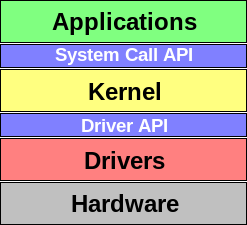
\includegraphics[width = 0.4\hsize]{./figures/esquema.png}
\caption{System Layers}
\label{fig:esquema1 de capas}
\end{figure}

Not all devices need driver installation. Those that are essential for the operation of a PC are included in the factory; This is the case of processors, disks and memories. When the device has an essential part and another does not, the support included by the system is basic; for example, when there are no drivers, the graphics cards show the windows, but not the special effects. It is as if the driver had only one basic dictionary available.\\

Figure 2 shows the different layers that exist from the highest level program to the hardware or device (low level), it is important to mention that you should not confuse driver with firmware; the second is inside the gray zone, because it is hardware.\\
\begin{figure}[H]
\centering
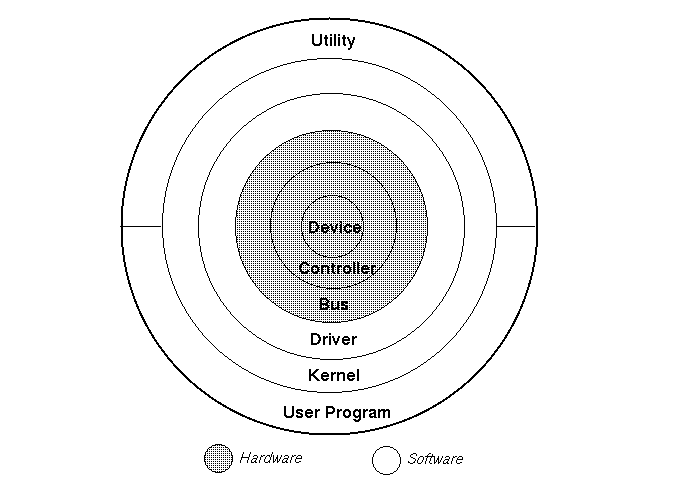
\includegraphics[width = 1\hsize]{./figures/esquema2.PNG}
\caption{System Modules}
\label{fig:modulos sistema}
\end{figure}

%https://www.softonic.com/articulos/que-son-los-drivers-controladores?fb_comment_id=1411452358895516_1657908310916585#f3615b11ca3aa8c


Drivers make work at such a basic level (low level) that the smallest error can destabilize the system. For example, if the system asks the driver of the graphic card to change the size of the screen and the driver does not establish communication with the card, a critical error will appear, which can render the computer useless.\\

To make a device usable there must be a driver present for it. So let us understand how an application accesses data from a device with the help of a driver. We will discuss the following four major entities, these major are based in figure 1.
\begin{itemize}
\item User-space application: This can be any simple utility like echo, or any complex application.
\item Device file: This is a special file that provides an interface for the driver. It is present in the file system as an ordinary file. The application can perform all supported operation on it, just like for an ordinary file. It can move, copy, delete, rename, read and write these device files.
\item Device driver: This is the software interface for the device and resides in the kernel space.
\item Device: This can be the actual device present at the hardware level, or a pseudo device.
\end{itemize}

\newpage

\section{Development environment}

To implement this project we used some tools that made easier the work. Some of the tools in our environment are:

\begin{itemize}
\item Sublime Text: very popular text editor that supports multiple programming languages. Some languages that can be used in this editor are: Python, Java, C, C++, PHP, ASM, and more.
\item GNU C/C++ Compiler: most important compiler for languages such as C and C++. In this project it was used to generate the necessary executables from the .c and .h files.
\item Arduino: open source platform which has the objective to bring an cheap option to learn about computing science.
\item Android Studio: program used to create an Android App. It has the option to debug using a tablet or a virtual device to check the status of the application. 
\item Makefiles: files that have a command list that will be executed in order to compile the files automatic.
\end{itemize}

\newpage

\section{Continuous learning attributes analysis}

For the resolution of this project, soft skills such as teamwork were worked, where a leader was assigned considering the requirement that was being sought at the time. We also sought to provide effective communication, first by obtaining the requirements of the system, then by designing the general model of the system and the way in which they communicate, and finally by implementing the different parts required. It was taken into account that each person is responsible for carrying out their tasks, communicating their progress and the obstacles encountered to find an effective solution as quickly as possible.

\newpage

\section{Program Design}

The program has 4 components: device driver, device library, interpreter and the android app. \\
The project's objective is to control the robot finger using a certain language to write some instructions. These instructions are necessary to make the robotic finger to move on a numeric keyboard and complete a PIN generated by the android app or a security pattern defined by the user. It's important to say that the app is capable of making three different views of the input, so the robotic finger can adjust the variables to fit the correct view. \\

The data flow of the project is shown below:
\begin{itemize}
\item The data will enter through the interpreter with the instructions written by the user that wants to generate a movement in the robotic finger.
\item These instructions are analyzed by the library that is in charge of writing a code for each type of instruction on the device. Each one has an unique code, so the hardware knows what action do.
\item The device takes this code sent by the user and transform it in an action to be executed on the robotic finger.
\end{itemize}

The interpreter has the job to take the input given by the user and transform it to computer language. The process consists in a parser to take each element and analyze it. The first step checks if the mnemonic of the instruction is correct to ensure that the input is correct. When it is analyzed, then it searches the argument. In this case the argument is an integer which says the amount of steps or spaces that the finger has to move. \\

The library consists of several methods that are capable of writing a specific code depending on the input generated by the user. Each of these codes has to be unique because the device has to read the operation on memory to execute the correct instruction. The objective is to make a modular project. When the tasks are separated the communication is easier between all the modules. With this idea, the tasks of writing on the device is assigned to the library and not to the interpreter or another method. \\

The driver probes searching for the device that wants to connect. When it finds the required device, the driver makes the initialization of the device to notify the operative system that the devices is ready to use. The main operations of a driver are write and read. In this project these operations are necessary to send the instructions to the device. When the device needs to finish the connection, the driver provides methods to do all the process and eliminate the register on the operative system, so there's no option to communicate to the device. \\

The embedded system used in the project is Arduino. For the hardware implementation the main components used are motors. The reason for this is that it's necessary the movement of the robotic finger through the tablet. \\


The details of the communication between the different modules in the system are shown in the figure below.

\begin{figure}[tb]
\centering 
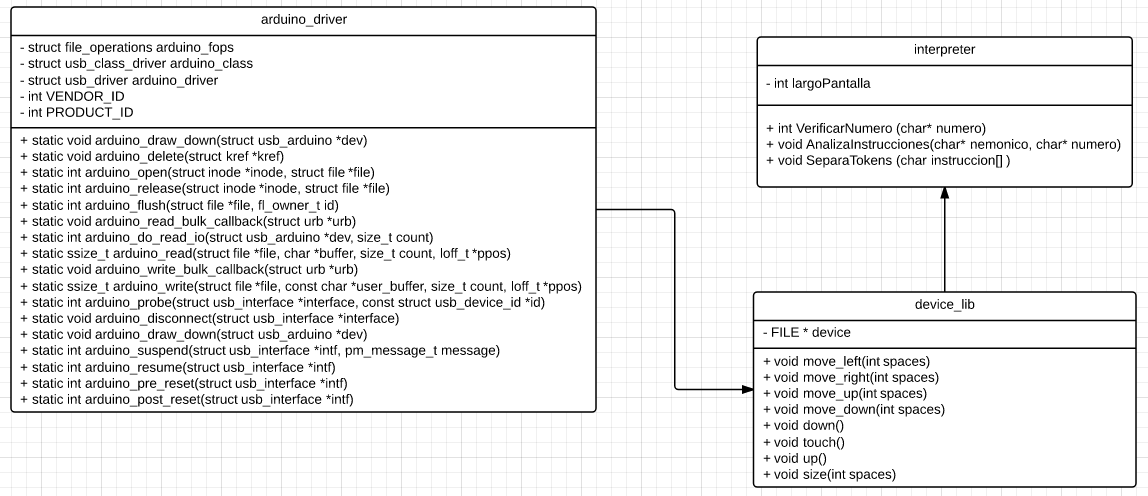
\includegraphics[width = 1\hsize]{./figures/UML.png}
\caption{UML Diagram for the project} % caption of the figure
\label{fig:umlfigure}
\end{figure}


\newpage

\section{How to use the program?}
\begin{enumerate}
\item Execute this command sudo rmmod cdc\_acm. Remove the factory Arduino driver
\item Execute this command cd driver \&\& make. Enter the driver folder and compile it
\item Execute this command sudo insmod arduino\_driver.ko .Insert the driver in the kernel
\item Execute this command sudo chmod a+rw /dev/arduino0. Read and write permissions
\item Generate the pin and pattern on movile device as follow image.
\begin{figure}[H]
\centering
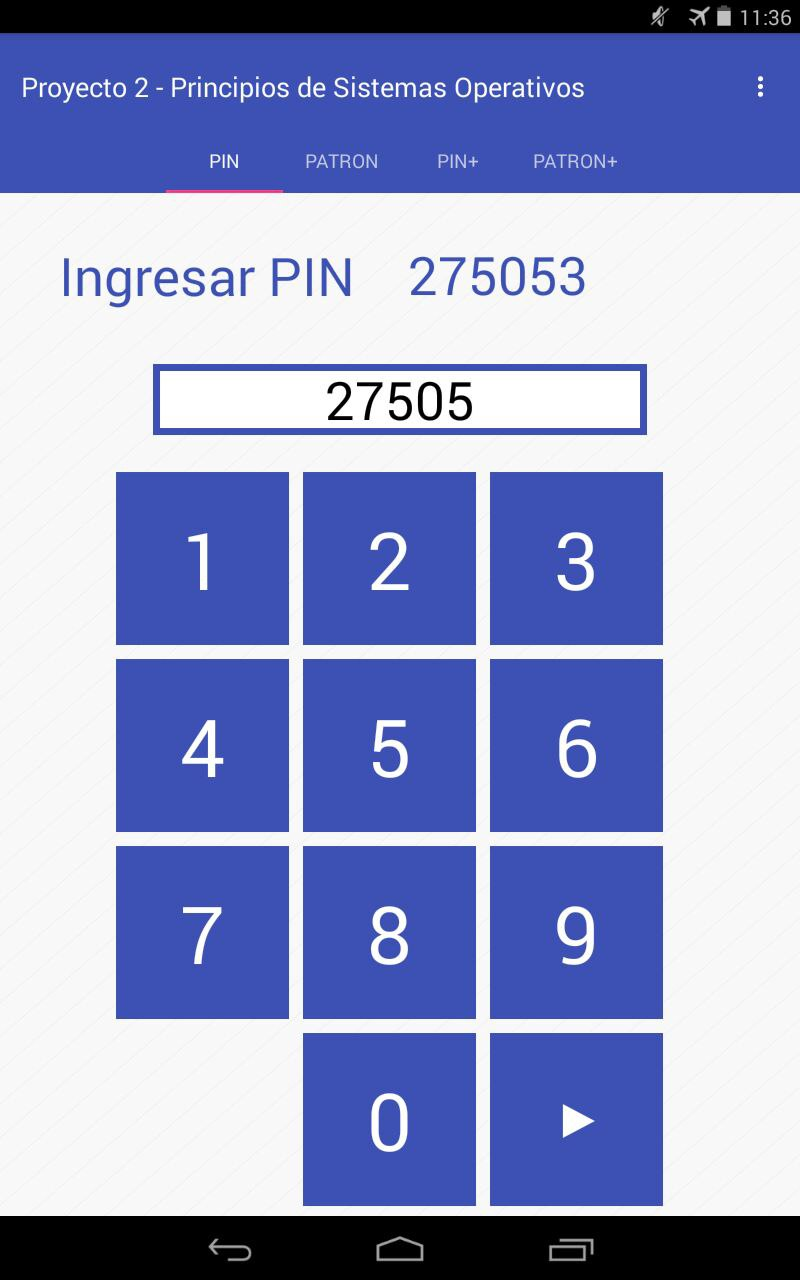
\includegraphics[width = 0.4\hsize]{./figures/pin.jpg}
\caption{Pin}
\label{fig:Generate}
\end{figure}

\begin{figure}[H]
\centering
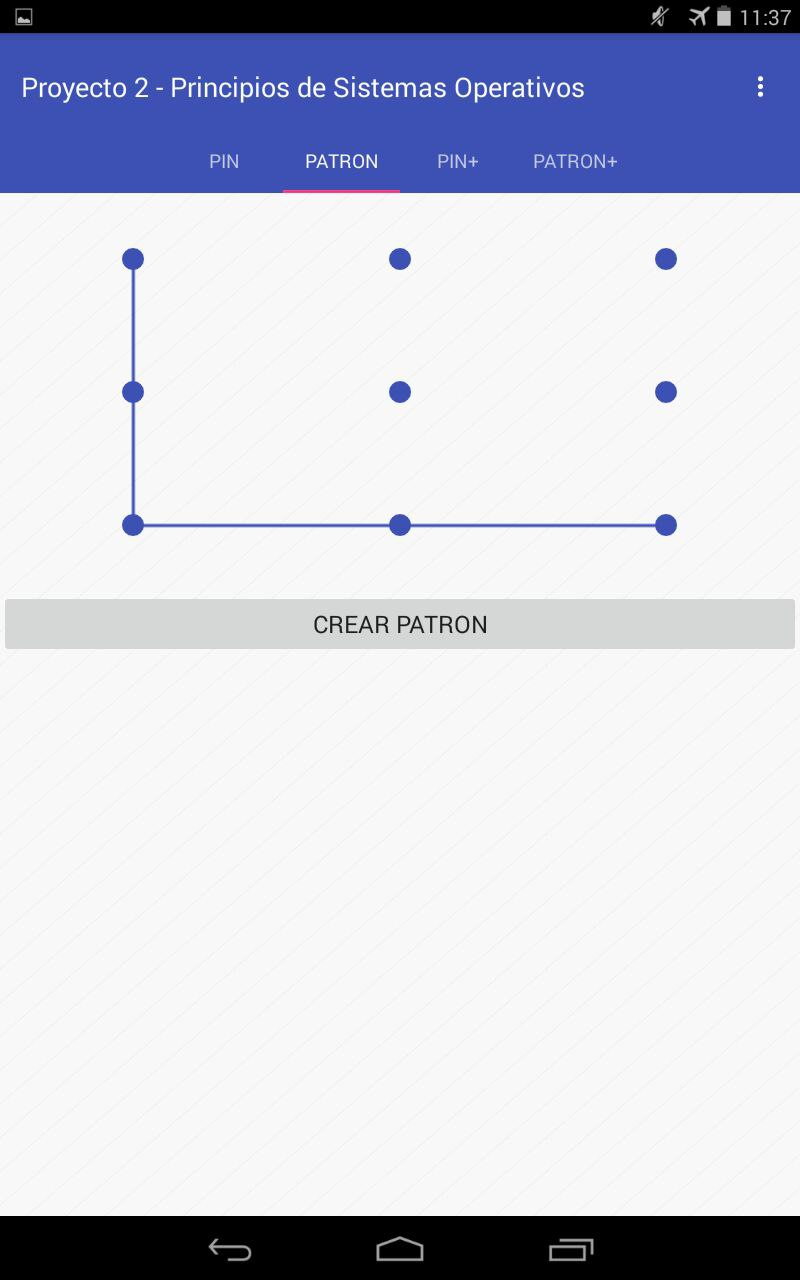
\includegraphics[width = 0.4\hsize]{./figures/patron.jpg}
\caption{Pattern}
\label{fig:Pattern}
\end{figure}

\item Execute this command ./interprete on the correct directory. It will show the follow image.
\begin{figure}[H]
\centering
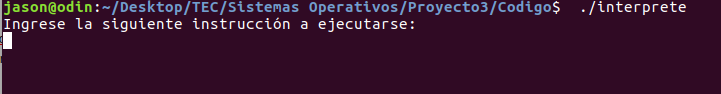
\includegraphics[width = 0.4\hsize]{./figures/interprete.png}
\caption{Interpreter}
\label{fig:esquema1 de capas}
\end{figure}

\item Type the instructions of lenguage.

\end{enumerate}


\newpage

\section{Students activity Logs}

\begin{table}[H]
\centering
\caption{My caption}
\label{my-label}
\begin{tabular}{ | m{7em} | m{7em} | m{16em} | m{4em} |}
\hline
\textbf{Member}                & \textbf{Activity}                            & \textbf{Description}                                                                                                                                                                                         & \textbf{Time (Hours)} \\
\hline
Jason, Jose, Luis, Carlos & UML Diagram                         & Meeting to discuss the UML diagram and the structure of the complete system.                                                                                                                        & 1:00         \\
\hline
Jason                    & Interpreter design                  & Research about the tokens for strings and creating the structure of the Interpreter's methods that allow the communication to the library.                                                          & 3:00         \\
\hline
Luis                     & Mobil App                           & Research about the Android Studio and it's variables, also about the libraries that allows the design of the pattern and numeric code.                                                              & 2:30         \\
\hline
Carlos                   & Hardware for Robotic Finger         & Get the components of the hardware and create the design of the robotic finger. Also, begin with the implementation of the structure base .                                                         & 8:00         \\
\hline
Jason                    & Interpreter and Programing Language & Define the structure of the programming language with the correct syntax structure and it's semantic structure. Implement the up, down and push function in the interpreter.                        & 3:00         \\
\hline
Jose                     & Arduino Driver                      & Research about the design of Linux driver that allows the communication with an specific device also research about the communication protocol of an Arduino.                                      & 3:30         \\
\hline
Jason                    & Interpreter                         & Define and implement the function of movement in any direction on the interpreter.                                                                                                                  & 2:30         \\
\hline

Luis                     & Library                             & Design and implement the functions that allows the writing bytes to the device into a library, It's writing in C language programming.                                                            & 2:00         \\
\hline

Jose                     & Arduino Driver                      & Implement the design of the structures and parameters that allows the identification of Arduino device. Also implement the methods to read and write data to the correct device.                    & 5:00         \\
\hline
\end{tabular}
\end{table}

\begin{table}[H]
\centering
\begin{tabular}{ | m{7em} | m{7em} | m{16em} | m{4em} |}
\hline
Carlos                   & Hardware                            & Creates the design of the movement in any direction with the servo motors and stepper motor, also use a pulley to perform the movement. All this is done through an Arduino device.                  &   8:00            \\
\hline
Luis                     & Mobil App                           & Creates the screens of the numeric codes with a random algorithm that creates a security password, also creates the screen of the pattern that allows to set a specific password define by the user. &  4:00 	\\           \hline
\end{tabular}
\end{table}


\newpage

\section{Project Final State}

\subsection*{Interpreter}

The final state of the interpreter is one hundred percent, it complies with identifying and verifying the sintaxys of the proposed language, as well as obtaining the data that the user wants to execute on the device.\\
\subsection*{Library}
The state of the library is one hundred percent, it receives the data of the interpreter and writes the data in file of the device.
\subsection*{App}
The state of the application is one hundred percent, it generates and verifies the pin, as well as the pattern.
\subsection*{Driver}
The status of the driver is one hundred percent, it performs the reception and sending of data to the arduino.
\subsection*{Robotic Finger}
The robotic finger is able to move and push the screen. If the finger is down, it's not always able to move. The functionality is around ninety percent.

\newpage

\section{Conclutions}

\begin{enumerate}
\item It is concluded that the drivers not only need to write and read from and to memory but that it is also important to establish a protocol to send and receive data from the device.

\item It is concluded that modularity makes a better distribution of tasks and generates independence between each stage of the project, which makes it more portable and facilitates debugging.

\item It is concluded that interpreter is a tool which facilitates the interaction of the user with the application, translating from an everyday language to an abstract one so that the driver can understand the instructions that he wants.



\end{enumerate}

\newpage

\section{Recomendations}

\begin{enumerate}
\item Tools such as Flex and Jack can be used to implement the interpreter and analyze the language instructions.
\item You can use data structures defined for each device and each depends of own protocol.
\item You can use libraries for graphic generation in the mobile application as DeviceLib. 
\item For the physical part you can use stepper motors to have better control of the movement in the two axes.
\end{enumerate}

% FIGURES

%\begin{figure}[tb]
%\centering 
%\includegraphics[width = 0.7\hsize]{./figures/imperial}
%\caption{This is a figure.} % caption of the figure
%\label{fig:imperial figure}
%\end{figure}
%Fig.~\ref{fig:imperial figure} shows the Imperial College logo. 

% TABLES

%\begin{table}[tb]
%\caption{Notation}
%\label{tab:notation}
%\centering
%\begin{tabular}{ll}
%Scalars & $x$\\
%Vectors & $\vec x$\\
%Matrices & $\mat X$\\
%Transpose & $\T$\\
%Inverse & $\inv$\\
%Real numbers & $\R$\\
%Expected values & $\E$\\
%\end{tabular}
%\end{table}
%Table~\ref{tab:notation} lists some notation with some useful shortcuts (see latex source code).
\newpage

\begin{thebibliography}{99}

\bibitem{c1} Fisher, T. (2017). What Is a Device Driver?. [online] Lifewire. Available at: https://www.lifewire.com/what-is-a-device-driver-2625796 [Accessed 24 Nov. 2017].

\bibitem{c2} Hope, C. (2017). What is a Device Driver?. [online] Computerhope.com. Available at: https://www.computerhope.com/jargon/d/driver.htm [Accessed 24 Nov. 2017].

\bibitem{c3} Docs.microsoft.com. (2017). What is a driver. [online] Available at: https://docs.microsoft.com/en-us/windows-hardware/drivers/gettingstarted/what-is-a-driver- [Accessed 24 Nov. 2017].

\end{thebibliography}

\end{document}
%%% Local Variables: 
%%% mode: latex
%%% TeX-master: t
%%% End: 
